%%% Template originaly created by Karol Kozioł (mail@karol-koziol.net) and modified for ShareLaTeX and
%%% Rafael de Lucena Valle use

\documentclass[a4paper,11pt]{article}

\usepackage[T1]{fontenc}
\usepackage[utf8]{inputenc}
\usepackage{graphicx}
\usepackage{xcolor}

\renewcommand\familydefault{\sfdefault}
\usepackage{tgheros}
\usepackage[defaultmono]{droidmono}

\usepackage{amsmath,amssymb,amsthm,textcomp}
\usepackage{enumerate}
\usepackage{multicol}
\usepackage{tikz}

\usepackage{geometry}
\geometry{total={210mm,297mm},
left=25mm,right=25mm,%
bindingoffset=0mm, top=20mm,bottom=20mm}


\linespread{1.3}

\newcommand{\linia}{\rule{\linewidth}{0.5pt}}

% custom theorems if needed
\newtheoremstyle{mytheor}
    {1ex}{1ex}{\normalfont}{0pt}{\scshape}{.}{1ex}
    {{\thmname{#1 }}{\thmnumber{#2}}{\thmnote{ (#3)}}}

\theoremstyle{mytheor}
\newtheorem{defi}{Definition}

% my own titles
\makeatletter
\renewcommand{\maketitle}{
\begin{center}
\vspace{2ex}
{\huge \textsc{\@title}}
\vspace{1ex}
\\
\linia\\
\@author \hfill \@date
\vspace{4ex}
\end{center}
}
\makeatother
%%%

% custom footers and headers
\usepackage{fancyhdr}
\usepackage{graphicx}
\usepackage{float}
\pagestyle{fancy}
\lhead{}
\chead{}
\rhead{}
\cfoot{}
\rfoot{Page \thepage}
\renewcommand{\headrulewidth}{0pt}
\renewcommand{\footrulewidth}{0pt}
%

% code listing settings
\usepackage{listings}
\lstset{
    language=Python,
    basicstyle=\ttfamily\scriptsize,
    aboveskip={1.0\baselineskip},
    belowskip={1.0\baselineskip},
    columns=fixed,
    extendedchars=true,
    breaklines=true,
    tabsize=4,
    prebreak=\raisebox{0ex}[0ex][0ex]{\ensuremath{\hookleftarrow}},
    frame=lines,
    showtabs=false,
    showspaces=false,
    showstringspaces=false,
    keywordstyle=\color[rgb]{0.627,0.126,0.941},
    commentstyle=\color[rgb]{0.133,0.545,0.133},
    stringstyle=\color[rgb]{01,0,0},
    numbers=left,
    numberstyle=\scriptsize,
    stepnumber=1,
    numbersep=10pt,
    captionpos=t,
    escapeinside={\%*}{*)}
}

%%%----------%%%----------%%%----------%%%----------%%%

\begin{document}

\title{Distributed Crypto Currency: Bitcoin}

\author{Rafael de Lucena Valle, Universidade Federal de Santa Catarina}

\date{30/06/2014}

\maketitle

\title{Bitcoin}

\section*{Definição}

O Bitcoin é uma moeda digital onde transações são enviados diretamente de uma parte a outra e utiliza algoritmos criptográficos para validar as transações e meios de recompensa para reduzir os ataques. Ao contrário das transações tradicionais que utilizam instituições financeiras como terceiro confiável no processo de pagamento eletrônico. Desta forma reduz custos entre transações e habilita tipos microtransações que não eram possíveis devido ao alto custo relativo.

Para prevenir o problema de duplo gasto, o Bitcoin propõe um servidor timestamp duma rede distribuída peer-to-peer que gere um uma ordem cronológica das transações. O sistema é seguro enquanto os nós honestos coletivamente controlarem mais CPU power que um grupo de atacantes. A idéia é fomentar nodos que ajudem a validar as transações, não precisando de uma instituição que garanta que não haja duplo-pagamento.
\cite{nakamoto2008bitcoin}
\section*{Moeda}
A moeda é uma cadeia de assinatura digitais, cada dono que transfere a moeda assina publicamente um hash da transação antiga e a chave pública do próximo dono e adiciona isso no final de cada moeda. Existe um problema na qual o pagador não pode verificar se o atual dono não gastou duplamente a moeda. Abaixo \ref{bitcoin} uma visão geral do Bitcoin.


\begin{figure}[H]
   \label{bitcoin}
   \centering
   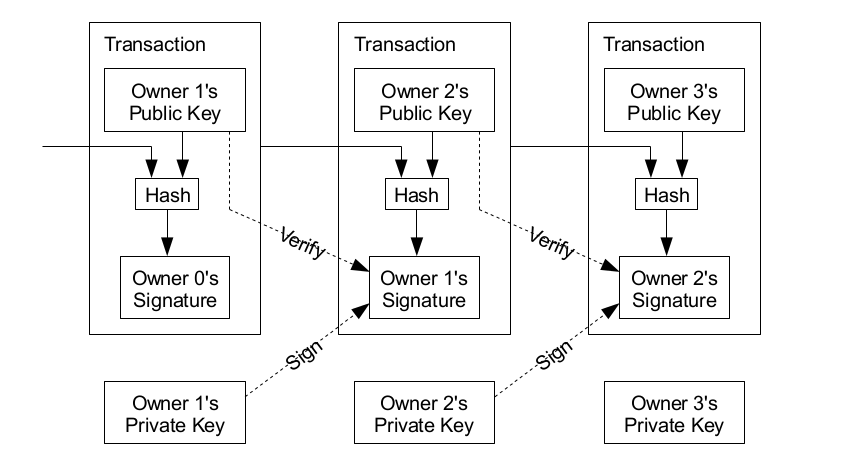
\includegraphics[width=0.8\textwidth]{images/coin.png}
   \caption{Modelo da moeda digital \cite{nakamoto2008bitcoin}.}
\end{figure}

\section*{Transações}
Para resolver o problema do gasto duplo o Bitcoin, as transações são publicamente anunciadas e são necessários participantes que concordem em uma história única da ordem em que são recebidas. O futuro dono precisa da prova que no momento da transação a maioria dos nós concordam que é o primeiro pagamento desta moeda do dono.

Para cifrar as transações o algoritmo utilizado é o  ECDSA, Assinatura Digital de Curvas Elípticas, assinando a alteração da propriedade possui as entradas: registros das transações antigas e a saída é um registro determinando o novo dono do Bitcoin, que será utilizado como entrada para futuras transações.

A solução do Bitcoin utiliza um servidor de timestamp que funciona gerando um hash do bloco de itens e publica este hash. Cada timestamp inclue o timestamp anterior formando uma cadeia.

Para implementar um servidor de timestamp distribuído é utilizado um sistema similar ao Hashcash, para proteger a rede e manter a rede decentralizada sem autoridade central. O trabalho requerido em média é exponencial ao número de bits zero. Uma vez que o trabalho satisfaz a prova de trabalho o bloco, a prova de trabalho é um voto por CPU.

Para compensar o aumento da velocidade de hardware durante o tempo, a dificuldade da prova de trabalho pode ser determinada alterando o número médio de blocos por hora. Os passos para executar a rede são:
\begin{itemize}
    \item Novas transações são comunicadas para todos os nós.
    \item Cada nó coleta novas transações para o bloco.
    \item Cada nó trabalha em encontrar a prova de trabalho de seu bloco.
    \item Quando um nó encontra um prova de trabalho, envia broadcast para todos os nodos.
    \item Nós aceitam o bloco apenas se todas as transações são validas e não foram gastos.
    \item Nós expressam a aceitação do bloco criando no próximo bloco da cadeia usando o hash de aceitação do bloco anterior.
\end{itemize}

Os nós sempre consideram a cadeia mais longa como correta no caso de dois nós fizeram broadcast simultâneo de diferentes versões do próximo bloco. Alguns podem receber uma ou outra primeiro, neste caso ele trabalha na primeira recebida porém salva a próxima caso a cadeira se torne maior. O broadcast necessita alcançar um número minimo de nós.

\section*{Mineração}
Para criar novas moedas é necessário que seja a primeira transação de um bloco.
\section*{Monetização}
\section*{Carteira Digital}

\bibliography{relatorio}{}
\bibliographystyle{plain}

\end{document}
